\documentclass[conference]{IEEEtran}
\IEEEoverridecommandlockouts
\usepackage{cite}
\usepackage{amsmath,amssymb,amsfonts}
\usepackage{graphicx}
\usepackage{textcomp}
\usepackage{xcolor}
\def\BibTeX{{\rm B\kern-.05em{\sc i\kern-.025em b}\kern-.08em
    T\kern-.1667em\lower.7ex\hbox{E}\kern-.125emX}}
\begin{document}

\title{Sentiment Analysis of Indonesian Mobile Banking App Reviews with a Fine-Tuned IndoBERT: Evidence from 134,910 Google Play Reviews}

\author{\IEEEauthorblockN{Author Name}
\IEEEauthorblockA{\textit{Department} \\
\textit{Institution}\\
City, Indonesia \\
email address}
}

\maketitle

\begin{abstract}
Mobile banking apps generate large volumes of public user feedback, but the reviews are written in informal Indonesian and may be dominated by organized campaigns instead of product experience. This paper analyzes 134,910 Google Play reviews of four Indonesian mobile banking apps (BRImo, myBCA, Livin' by Mandiri, and wondr by BNI) posted between January and August 2026. We fine-tune IndoBERT for three-class sentiment classification with 1,900 manually labeled reviews (1,400 for training and 500 for testing) and evaluate it with grouped cross-validation and a random held-out test set. The model reaches a test macro-F1 of 0.944 (95 percent interval 0.820 to 0.979), and 0.826 on test reviews whose text is absent from the training data, outperforming a TF-IDF baseline. Predicted sentiment is corrected for classifier error and combined with a manually labeled topic sample. Livin' and myBCA are predominantly negative, whereas BRImo and wondr are predominantly positive. The surge of negative Livin' reviews in August 2026 is mostly a protest campaign about account blocking: an estimated 59 to 71 percent of negative reviews that month concern bank policy, while technical complaints remain at their usual level. We find no consistent evidence that sentiment improves with newer app versions. The results show that text-based sentiment analysis should be complemented by topic analysis to separate product feedback from campaign activity.
\end{abstract}

\begin{IEEEkeywords}
sentiment analysis, IndoBERT, Indonesian language, mobile banking, app reviews, prevalence estimation
\end{IEEEkeywords}

\section{Introduction}
Mobile banking has become a primary channel through which Indonesian customers transfer money, pay bills, and open accounts. The apps of the largest banks are distributed through Google Play, where every user can publish a public, timestamped review attributed to a specific app version. App store reviews are therefore a continuous and inexpensive source of customer feedback, and their analysis has become an established line of software engineering research \cite{b1,b2}.

Turning such reviews into reliable evidence is difficult for four reasons. First, the text is informal Indonesian with abbreviations, regional words, misspellings, and emoji. Second, labeled data are scarce, and the neutral class is small relative to the negative and positive classes. Third, review streams are not only product feedback: organized campaigns, such as boycotts or prize-related review drives, can generate large volumes of reviews that say little about app quality. Fourth, when predicted labels are aggregated into proportions, the classifier's errors bias the proportions, which matters whenever apps or periods are compared.

Pretrained language models address the first two problems. BERT \cite{b3} and its Indonesian variants \cite{b4} can be fine-tuned from a few hundred or thousand labeled examples. The remaining two problems are not solved by a better classifier and require explicit treatment in the analysis.

This paper studies the following research questions.
\begin{itemize}
\item \textbf{RQ1.} How accurately can a fine-tuned IndoBERT classify the sentiment of Indonesian mobile banking reviews when labeled data are limited, and how does it compare with a lexical baseline?
\item \textbf{RQ2.} What is the distribution of negative, neutral, and positive reviews across apps and months once classifier error is taken into account?
\item \textbf{RQ3.} How much of an observed surge in negative reviews reflects app problems rather than other topics, and does sentiment vary with the installed app version?
\end{itemize}

The contributions are as follows. We describe a collection, labeling, and sampling protocol for app reviews that keeps a random test set free of model-based selection. We evaluate IndoBERT against a TF-IDF baseline with group-aware cross-validation and bootstrap intervals that resample whole texts. We estimate sentiment proportions for a census of 134,910 reviews, corrected for classifier error. Finally, we show with a manually labeled topic sample that the largest sentiment anomaly in the data is a policy-related campaign, and we quantify its size.

The remainder of the paper is organized as follows. Section~\ref{sec:related} reviews related work. Sections~\ref{sec:data} to~\ref{sec:methods} describe the data, the annotation, and the methods. Section~\ref{sec:results} presents the results, which are discussed in Section~\ref{sec:discussion}. Section~\ref{sec:limits} lists limitations, and Section~\ref{sec:conclusion} concludes.

\section{Related Work}\label{sec:related}
\subsection{App Review Analysis}
Early empirical work on app store feedback showed that reviews are numerous and that review activity clusters shortly after new releases \cite{b1}. A survey of app store analysis places review mining among several lines of research that use app store data for software engineering \cite{b2}. Studies of reviews generally treat each review as an independent observation, whereas in practice reviews are repeated, edited, and sometimes organized, which motivates the data audit and the topic analysis in this paper.

\subsection{Indonesian Language Models and Fine-Tuning}
BERT \cite{b3} pretrains a bidirectional transformer encoder with a masked-language-model objective and is adapted to classification by fine-tuning. IndoNLU provides a benchmark and pretrained IndoBERT models for Indonesian \cite{b4}, and IndoLEM provides a separate IndoBERT model and benchmark \cite{b5}. Fine-tuning strategies for text classification have been studied systematically \cite{b6}, and fine-tuning on small datasets is known to be sensitive to the random seed \cite{b7}, which we address by averaging several seeds and reporting seed-to-seed variation. Continued pretraining on unlabeled in-domain text can improve downstream performance \cite{b8}; we test this idea on the review corpus.

\subsection{Prevalence Estimation under Classifier Error}
Estimating the share of each class in a population from the predictions of an imperfect classifier is the problem of quantification \cite{b9}. In epidemiology, the correction of an observed prevalence for known error rates dates back to the Rogan--Gladen estimator \cite{b10}. In machine learning, the same idea underlies black-box shift estimation, which inverts a confusion matrix estimated on held-out data \cite{b11}. We apply this correction to the review population.

\subsection{LLM-Assisted Annotation}
Large language models have been reported to match or exceed crowd workers on several text annotation tasks \cite{b12}. We use an LLM to apply written annotation guidelines at scale and quantify the agreement with an independent human annotator, instead of treating the LLM labels as ground truth.

\section{Data Collection}\label{sec:data}
Reviews were collected at the end of October 2026 with the open-source google-play-scraper library, using the Indonesian language and country settings. For each app, reviews are requested newest-first with retries and exponential backoff until the oldest review in a batch lies two days before the study period; each scan is logged, and the log records whether the start of the period was reached, which was the case for all four apps. The scraper returns naive timestamps in the timezone of the machine that ran it (UTC); they were converted to Asia/Jakarta time so that month boundaries follow Indonesian time. Only the review text, star rating, timestamp, app version, and number of helpful votes were retained; user names and avatars were not stored.

The scan yielded 162,400 reviews, of which 134,910 fall in the study period (1 January to 31 August 2026), have a unique review identifier, and contain text. Table~\ref{tab:population} summarizes the population. Version information is missing for 10 to 36 percent of the reviews depending on the app. In the population, 41.8 percent of the reviews share their exact text with at least one other review, and 3.3 percent are shorter than three characters. Short and repeated reviews were kept, because they are a substantial part of what the model must score.

An audit of the monthly counts flagged one anomaly: Livin' received 18,463 reviews in August 2026, which is 8.7 times its monthly median.

\begin{table}[htbp]
\caption{Review Population by App}
\begin{center}
\footnotesize
\begin{tabular}{|l|r|r|r|}
\hline
\textbf{App} & \textbf{Reviews} & \textbf{With version (\%)} & \textbf{Largest month} \\
\hline
BRImo & 59,506 & 81.6 & 9,067 (April) \\
Livin' by Mandiri & 35,968 & 64.2 & 18,463 (August) \\
wondr by BNI & 30,604 & 90.0 & 4,491 (March) \\
myBCA & 8,832 & 77.9 & 1,520 (March) \\
\hline
\textbf{Total} & \textbf{134,910} & & \\
\hline
\end{tabular}
\label{tab:population}
\end{center}
\end{table}

\section{Annotation and Dataset Construction}\label{sec:annotation}
\subsection{Label Scheme}
Each review is assigned one of three classes from its text alone; the star rating and the date were hidden from the labeling sheet. Reviews that express satisfaction, praise, gratitude, or a recommendation are positive. Reviews that report a failure or a problem, express frustration, or ask a question that states a failure are negative; a review that praises the app and then states a concrete complaint is also negative. Neutral reviews contain no evaluation: a stand-alone ``ok'', a procedural or situational question without a stated failure, a feature request without a complaint, a hope or a prayer, or a statement that the reviewer has just started using the app. A request that implies a defect or a burden, such as a request to raise a transfer limit, is negative. Decisions on borderline cases were fixed in written guidelines before the main labeling and flagged with an uncertainty indicator when the call was close.

\subsection{Sampling}
Table~\ref{tab:splits} shows the labeled data. The test set is a simple random sample of 125 reviews per app. The training pool of the first round uses 250 reviews per app with equal quotas across months and at most two copies of an identical text, so that frequent one-word reviews do not dominate. A second round of 400 reviews was selected with the first-round model: per app, 40 reviews with the highest neutral probability (excluding variants of ``ok''), 40 with the highest predictive entropy, and 20 random reviews. Reviews selected in this way were added to the training pool only, so the test set remains free of model-based selection.

\begin{table}[htbp]
\caption{Labeled Data (negative / neutral / positive)}
\begin{center}
\footnotesize
\begin{tabular}{|l|r|r|}
\hline
\textbf{Set} & \textbf{Reviews} & \textbf{Neg. / Neu. / Pos.} \\
\hline
Test (random) & 500 & 254 / 29 / 217 \\
Training pool, round 1 & 1,000 & 520 / 42 / 438 \\
Training pool, round 2 (targeted) & 400 & 111 / 212 / 77 \\
\hline
\textbf{Training pool total} & \textbf{1,400} & 631 / 254 / 515 \\
\hline
\end{tabular}
\label{tab:splits}
\end{center}
\end{table}

\subsection{Annotation Procedure and Agreement}
The labels were assigned with a large language model (Claude, Anthropic) that applied the written guidelines, and the labeled sheets were checked for consistency: identical texts must carry identical labels, and lexical scans flagged labels that contradicted obvious cues in the text, which led to corrections. An independent human annotator labeled 190 reviews without seeing the model labels: 100 random reviews with a confident label and the 90 reviews marked as uncertain. Agreement measured with Cohen's kappa \cite{b13} was 0.88 (94 percent raw agreement; linearly weighted kappa 0.93) on the confident reviews, which is almost perfect on the scale of Landis and Koch \cite{b14}, and 0.33 (53 percent agreement) on the uncertain reviews, which is fair. The disagreements concentrated on three kinds of reviews: praise followed by a complaint, requests and suggestions, and situational questions. The decisions on these categories were made by the research team after the agreement analysis and applied to the whole data set. The resulting labels follow the conventions of this study, and the agreement on borderline reviews shows that other reasonable conventions exist.

\section{Methods}\label{sec:methods}
\subsection{Text Versions}
Four text versions were compared in a first round: the raw text (A); light normalization (B), which applies Unicode NFKC, removes zero-width characters, links, and mentions, shortens runs of three or more identical letters or symbols to two (digits are untouched), and normalizes whitespace; B plus a dictionary of 70 common abbreviations and slang forms (C); and B with six sentiment-bearing emoji replaced by words (D). Identical texts are grouped by a key that lowercases the text and removes punctuation.

\subsection{Models}
The baseline combines word n-grams (1 to 2) and character n-grams (3 to 5, within word boundaries) with TF-IDF weighting and class-balanced logistic regression, implemented with scikit-learn \cite{b15}; the regularization strength is chosen from $\{1,3,10\}$ by pooled out-of-fold macro-F1, which slightly favors the baseline.

The main model is the \texttt{indobert-base-p1} model of the IndoBenchmark project \cite{b4} with a linear classification head, fine-tuned with AdamW \cite{b16} using the Transformers \cite{b17} and PyTorch \cite{b18} libraries. The learning rate is $2\times10^{-5}$ with 10 percent linear warmup and linear decay, weight decay is 0.01, the batch size is 16, the number of epochs is four, the maximum sequence length is 128 (the longest review has 118 tokens), and gradients are clipped at 1.0. The cross-entropy loss is weighted by $(n/(Kn_k))^{0.5}$, where $n_k$ is the number of training reviews of class $k$ and $K=3$, which softens the effect of class imbalance. Five-fold cross-validation was repeated with three seeds, so each prediction is the average of three models, and the final population scores average all 15 fold models. We also tested continued pretraining with the masked-language-model objective on 81,874 unique review texts (all texts that occur in the test set were excluded) for two epochs. The released checkpoint contains no masked-language-model head, so the head was newly initialized.

\subsection{Evaluation Protocol}
Folds were built with stratified group $k$-fold, with identical texts forming a group, so that a text never appears in two folds. Macro-F1 is the main metric,
\begin{equation}
F_{1}^{\text{macro}}=\frac{1}{K}\sum_{k=1}^{K}\frac{2P_kR_k}{P_k+R_k},\label{eq:f1}
\end{equation}
where $P_k$ and $R_k$ are the precision and recall of class $k$. Confidence intervals are percentile intervals from 1,000 bootstrap replicates \cite{b19} that resample whole text groups; differences between models use the same replicates for both models (paired bootstrap). Model selection used pooled out-of-fold predictions only. The test set was evaluated once, after the configuration was fixed.

\subsection{Prevalence Estimation under Classifier Error}
Let $R$ be the $K\times K$ matrix with $R_{ij}=P(\hat{y}=j\mid y=i)$, estimated from the test confusion matrix, and let $\hat{q}$ be the predicted class shares of a group of reviews. The true shares $\pi$ satisfy $q=R^{\top}\pi$, and we estimate
\begin{equation}
\hat{\pi}=\arg\min_{\pi\ge 0,\ \mathbf{1}^{\top}\pi=1}\left\lVert R^{\top}\pi-\hat{q}\right\rVert_2^2,\label{eq:correction}
\end{equation}
which is solved by non-negative least squares \cite{b20} with the sum constraint appended as a heavily weighted row. Intervals come from resampling the test set by text group and recomputing $R$, so they reflect classifier uncertainty only; the reviews form a census of the collected period and have no sampling error with respect to it. The correction assumes that $R$ measured on the test set holds for the entire population. Intervals for observed proportions of a sample, such as version-level shares, use the Wilson method \cite{b21}.

\subsection{Topic Analysis of Livin' Reviews}
To quantify the August anomaly we manually labeled the topic of 400 randomly drawn Livin' reviews that were predicted negative: 300 from August and 100 from January to July. The topics are bank policy and boycott (account blocking, protest), app technical problems (login, verification, crashes, slowness), service and transactions (failed transfers, deductions, fees, customer service), and generic or other. A broad definition of the policy topic additionally counts generic insults directed at the bank. Topics were labeled without knowledge of the month or version. Counts for the population are obtained by scaling the sample shares by the number of predicted-negative reviews in the corresponding period.

\subsection{Version Analysis}
For reviews with a version, versions of an app are ranked by their numerical order, and a logistic regression of the predicted negative label on the version rank $r_v$ with month fixed effects $\alpha_m$ is estimated for each app,
\begin{equation}
\operatorname{logit}P(\hat{y}_i=\text{negative})=\alpha_{m(i)}+\beta\,r_{v(i)},\label{eq:logit}
\end{equation}
where $e^{\beta}$ is the odds ratio per version step holding the calendar month constant. The correlation between version rank and month is reported as a diagnostic, because a high value means the two cannot be separated well.

\section{Results}\label{sec:results}
\subsection{Classifier Performance (RQ1)}
\textit{Cross-validation.} Table~\ref{tab:cv} reports pooled out-of-fold results on the 1,400-review training pool. IndoBERT reaches a macro-F1 of 0.897 against 0.861 for the best baseline; the paired macro-F1 difference between the baseline and IndoBERT is $-0.036$ (95 percent interval $-0.056$ to $-0.017$), and the F1 of the neutral class is 0.830 against 0.781. These pooled figures are not estimates of population performance, because the pool contains model-targeted reviews and an 18 percent share of neutral reviews. On the 1,000 reviews of the first round, which were drawn without model targeting, IndoBERT reaches a macro-F1 of 0.865 (neutral F1 0.658) and the baseline 0.804 (neutral F1 0.525). The second labeling round raised the baseline on these reviews from 0.762 to 0.804 but left IndoBERT essentially unchanged (0.863 to 0.870 across runs).

\begin{table}[htbp]
\caption{Pooled Out-of-Fold Results (1,400 Reviews, Five Folds)}
\begin{center}
\footnotesize
\begin{tabular}{|l|c|c|c|c|}
\hline
\textbf{Model} & \textbf{Macro-F1 (95\% CI)} & \textbf{Neg.} & \textbf{Neu.} & \textbf{Pos.} \\
\hline
IndoBERT & 0.897 (0.879--0.915) & 0.937 & 0.830 & 0.926 \\
TF-IDF + LR & 0.861 (0.840--0.880) & 0.905 & 0.781 & 0.898 \\
\hline
\multicolumn{5}{l}{F1 by class in the last three columns. Three seeds for IndoBERT.}
\end{tabular}
\label{tab:cv}
\end{center}
\end{table}

\textit{Preprocessing and continued pretraining.} Table~\ref{tab:variants} compares the variants in the first round (one seed, 1,000 reviews). None differs from the raw text beyond bootstrap uncertainty (all paired intervals include zero), and the seed-to-seed variation of the same configuration is about 0.02. Neither the abbreviation dictionary, the emoji replacement, nor continued pretraining improved on light normalization, which was used throughout. Because the masked-language-model head was newly initialized, the continued pretraining result is conservative.

\begin{table}[htbp]
\caption{Text Versions and Continued Pretraining (First Round)}
\begin{center}
\footnotesize
\begin{tabular}{|l|c|}
\hline
\textbf{Variant} & \textbf{Macro-F1} \\
\hline
A, raw text & 0.857 \\
B, light normalization & 0.870 \\
C, B plus abbreviation dictionary & 0.840 \\
D, B plus emoji replaced by words & 0.844 \\
B with continued pretraining & 0.853 \\
\hline
\end{tabular}
\label{tab:variants}
\end{center}
\end{table}

\textit{Learning curve.} Fig.~\ref{fig:learning} shows that out-of-fold macro-F1 increases from 0.660 to 0.852 as the training data per fold grow from 200 to 800 reviews. The last increment ($+0.021$) is of the same size as the seed-to-seed variation, so additional random labels would add little to the overall score.

\begin{figure}[htbp]
\centerline{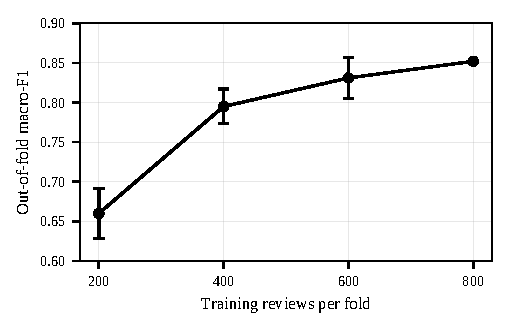
\includegraphics[width=\columnwidth]{figures/fig_learning_curve.pdf}}
\caption{Learning curve of IndoBERT on the first-round pool (mean and standard deviation over three repetitions of the subsampling).}
\label{fig:learning}
\end{figure}

\textit{Held-out test set.} Table~\ref{tab:test} reports the test results. The macro-F1 on all 500 reviews is 0.944 (accuracy 0.974). Restricted to the 375 test reviews whose text does not occur in the training pool, the macro-F1 is 0.826 and the neutral F1 0.533, which measures generalization to unseen text; the first view reflects the population as a whole, in which 41.8 percent of reviews are repeated texts. On the 472 reviews with a confident label the macro-F1 is 0.980. Of the 13 misclassified test reviews, eight belong to the 28 reviews marked as uncertain. The confusion matrix has the rows (true class) negative 250/2/2, neutral 3/24/2, and positive 4/0/213, which gives the error rates used in the correction below: 10.3 percent of neutral reviews are predicted negative and 6.9 percent positive, whereas confusion between negative and positive is at most 1.8 percent. The neutral class has only 29 test reviews, so its estimates, and every quantity derived from them, are rough.

\begin{table}[htbp]
\caption{Test Results (Held-Out Random Sample)}
\begin{center}
\footnotesize
\begin{tabular}{|l|r|c|c|}
\hline
\textbf{View} & \textbf{n} & \textbf{Macro-F1 (95\% CI)} & \textbf{Neu. F1} \\
\hline
All test reviews & 500 & 0.944 (0.820--0.979) & 0.873 \\
Text not in training pool & 375 & 0.826 (0.695--0.923) & 0.533 \\
Confident labels only & 472 & 0.980 (0.865--0.998) & 0.958 \\
\hline
\end{tabular}
\label{tab:test}
\end{center}
\end{table}

\subsection{Sentiment by App (RQ2)}
Table~\ref{tab:shares} and Fig.~\ref{fig:shares} present the corrected sentiment shares for all 134,910 reviews. Two apps are predominantly negative (Livin' 0.702, myBCA 0.644) and two are predominantly positive (positive shares of 0.645 for BRImo and 0.668 for wondr). The ordering is identical for the uncorrected predicted shares; the correction lowers the negative shares of BRImo and wondr by about 1.5 points, because the model sometimes assigns neutral reviews to the negative class. Neutral shares are small (4 to 8 percent) with wide intervals and should not be compared across apps. The model's maximum class probability was below 0.6 for 0.7 to 1.2 percent of the reviews.

\begin{table}[htbp]
\caption{Corrected Sentiment Shares by App (95\% Interval)}
\begin{center}
\scriptsize
\setlength{\tabcolsep}{2.5pt}
\begin{tabular}{|l|c|c|c|}
\hline
\textbf{App} & \textbf{Negative} & \textbf{Neutral} & \textbf{Positive} \\
\hline
BRImo & 0.289 (0.245--0.303) & 0.066 (0.056--0.137) & 0.645 (0.611--0.661) \\
Livin' & 0.702 (0.668--0.716) & 0.043 (0.031--0.090) & 0.255 (0.233--0.264) \\
myBCA & 0.644 (0.598--0.658) & 0.066 (0.053--0.138) & 0.290 (0.257--0.301) \\
wondr & 0.253 (0.200--0.268) & 0.079 (0.067--0.165) & 0.668 (0.627--0.685) \\
\hline
\end{tabular}
\label{tab:shares}
\end{center}
\end{table}

\begin{figure}[htbp]
\centerline{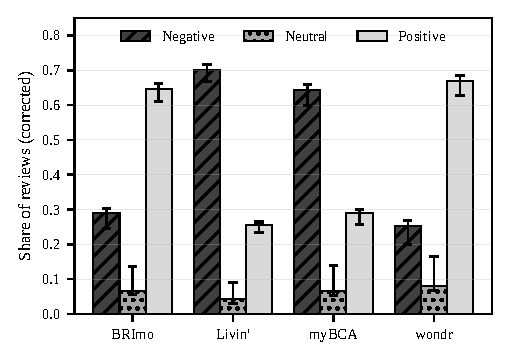
\includegraphics[width=\columnwidth]{figures/fig_app_shares.pdf}}
\caption{Corrected sentiment shares by app with 95 percent intervals from resampling the test set.}
\label{fig:shares}
\end{figure}

\subsection{Monthly Dynamics and the Livin' August Cluster (RQ3)}
Fig.~\ref{fig:monthly} shows the corrected negative share by month. BRImo (0.21 to 0.35), wondr (0.20 to 0.32), and myBCA (0.55 to 0.72) stay within stable ranges. Livin' is volatile: its monthly volume was 1,456, 1,637, 5,372, 2,499, 1,767, 1,448, 3,326, and 18,463 reviews from January to August, and its negative share ranged from 0.31 in July to 0.92 in August. Keywords for promotions and prize draws occur in at most 0.3 percent of the reviews in any app and month, so incentivized reviews do not explain the volume peaks in March and July, which remain unexplained.

\begin{figure}[htbp]
\centerline{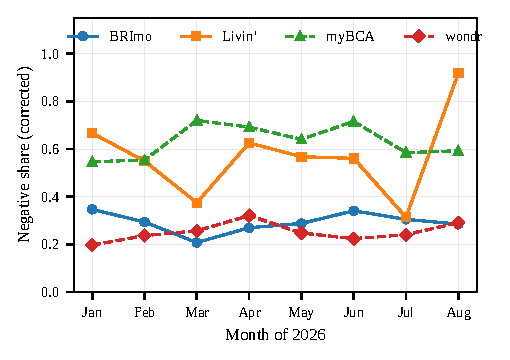
\includegraphics[width=\columnwidth]{figures/fig_monthly_negative.pdf}}
\caption{Corrected negative share by app and month in 2026 (point estimates).}
\label{fig:monthly}
\end{figure}

\textit{Keyword screen.} A keyword pattern for account blocking, boycott, and law enforcement flags 5,214 Livin' reviews (28 percent of the Livin' reviews in August) and fewer than 25 reviews in each other app; 99 percent of the flagged reviews are predicted negative. In a random sample of 15 flagged reviews, 14 were relevant, but reviews that mention blocking in policy terms without the pattern's keywords were missed, so the screen has limited recall. We therefore relied on the manual topic sample.

\textit{Topic sample.} Table~\ref{tab:topics} shows the topic composition of predicted-negative Livin' reviews. In January to July 87 percent of the negative reviews concern technical problems and 2 percent bank policy. In August 59 percent (95 percent interval 54 to 65) concern bank policy, 71 percent (66 to 76) under the broad definition, and only 7 percent technical problems.

\begin{table}[htbp]
\caption{Topic of Predicted-Negative Livin' Reviews}
\begin{center}
\footnotesize
\begin{tabular}{|l|c|c|}
\hline
\textbf{Topic} & \textbf{Jan.--Jul. (n = 100)} & \textbf{Aug. (n = 300)} \\
\hline
Bank policy and boycott & 2\% (0.6--7\%) & 59\% (54--65\%) \\
\ \ broad definition & 2\% & 71\% (66--76\%) \\
App technical problems & 87\% & 7\% \\
Generic or other & 3\% & 29\% \\
Service and transactions & 8\% & 5\% \\
\hline
\end{tabular}
\label{tab:topics}
\end{center}
\end{table}

Scaling the sample shares to the population, an estimated 9,900 (narrow definition) to 11,900 (broad definition) of the August reviews concern bank policy. Removing them, the share of negative predictions of Livin' in August falls from 0.91 to 0.80 (narrow) or 0.74 (broad), whereas it remains 0.48 in January to July; if all generic insults are removed as well, the August share is about 0.53. The August share without the campaign therefore lies between roughly 0.53 and 0.80, depending on the treatment of generic insults. Over the whole period, the Livin' share of negative predictions is 0.55 to 0.58 without policy reviews against 0.70 with all reviews, so Livin' remains more negative than BRImo and wondr. The number of technical complaints is approximately unchanged: about 1,050 per month from January to July against an estimated 1,100 in August (roughly 740 to 1,700 given the sampling uncertainty of the topic sample). The August surge is therefore not evidence of a decline in app quality.

\subsection{App Versions (RQ3)}
The version is the version installed on the reviewer's device, not the version current at the time of the review; old versions receive reviews until the end of the period, and reviewers on very old versions are a self-selected group. Reviews without a version are more often negative than reviews with a version (predicted negative share 54 versus 24 percent for wondr, 80 versus 64 percent for Livin', 37 versus 29 percent for BRImo, and 68 versus 64 percent for myBCA), and only 51 percent of the Livin' reviews of August carry a version, against 75 to 81 percent in other months.

\begin{figure}[htbp]
\centerline{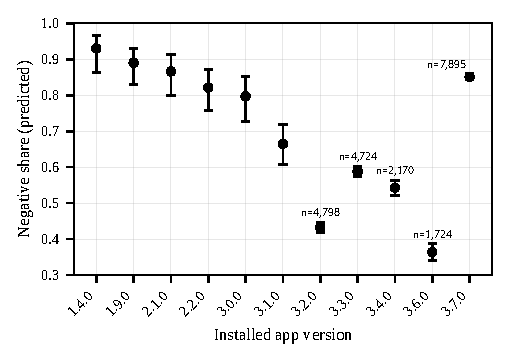
\includegraphics[width=\columnwidth]{figures/fig_livin_versions.pdf}}
\caption{Share of negative predictions by installed Livin' version (versions with at least 100 reviews; 95 percent Wilson intervals).}
\label{fig:versions}
\end{figure}

Fig.~\ref{fig:versions} shows that the negative share of Livin' is high for old versions, falls from 0.59 (3.3.0) to 0.36 (3.6.0), and rises to 0.85 for version 3.7.0, which has 7,895 reviews (34 percent of the Livin' reviews with a version) and was first reviewed on 15 July. In the August topic sample, 57 percent of the 3.7.0 reviews (61 of 108) concern bank policy and 9 percent (10 of 108) technical problems, similar to reviews without a version (59 percent policy, 160 reviews) and to other versions (69 percent, 32 reviews). The high negativity of 3.7.0 is therefore largely attributable to the campaign and not to the version. Among the other apps, version 2.15.1 of myBCA (0.75, 1,444 reviews) and 2.17.1 (0.70, 898 reviews) are well above neighboring versions, the share of BRImo falls to 0.22 for 2.95.1 and rises to 0.39 for 2.96.0, and the share of wondr rises slightly from 0.22 to 0.28 over its four versions with at least 100 reviews.

Table~\ref{tab:trend} reports the regression of Eq.~\eqref{eq:logit}. The odds ratios per version step are close to one, and version rank is correlated with calendar month at 0.23 to 0.83. Restricting the analysis to versions with at least 100 reviews gives odds ratios of 0.975, 1.028, 1.152, and 1.291 for BRImo, Livin', myBCA, and wondr, with correlations between version rank and month of 0.89 to 0.94 for three of the four apps. The direction therefore depends on the specification, and we find no consistent evidence that sentiment improves with newer versions in any app.

\begin{table}[htbp]
\caption{Odds Ratio of a Negative Prediction per Version Step}
\begin{center}
\footnotesize
\begin{tabular}{|l|c|c|c|}
\hline
\textbf{App} & \textbf{Versions} & \textbf{OR (95\% CI)} & \textbf{Corr. with month} \\
\hline
BRImo & 107 & 0.972 (0.969--0.976) & 0.47 \\
Livin' & 28 & 0.987 (0.976--0.999) & 0.23 \\
myBCA & 59 & 1.007 (0.995--1.018) & 0.57 \\
wondr & 15 & 1.006 (0.957--1.058) & 0.83 \\
\hline
\end{tabular}
\label{tab:trend}
\end{center}
\end{table}

\subsection{Validity Checks}
Star ratings were never used by the model or the labels. The mean rating decreases from positive to negative predictions: 4.87 for positive, 4.56 for neutral, and 1.86 for negative reviews; the neutral class contains many short approvals that usually carry five stars. A total of 6,548 reviews are predicted negative with five stars (18.7 percent of the predicted-negative reviews of BRImo, 15.2 percent for wondr, 8.6 percent for myBCA, and 5.7 percent for Livin'). In a random sample of 20, about 14 were genuine complaints with a high rating, about three were model errors, and the rest were ambiguous, so ratings alone would misclassify a substantial share of complaints. A total of 1,153 reviews are predicted positive with one or two stars (8.2 percent of the positive predictions of Livin' and about 1 percent elsewhere); in a random sample of 20, about a third were model errors on short slang, misspelled, or emoji-only text, and the rest were positive text with a protest rating or ambiguous text. This stratum is below 1 percent of the population. Finally, 1,137 reviews (0.84 percent) consist only of emoji and all are predicted positive; an emoji lookup classifies 904 of them as positive, 65 as negative, and 168 as unclear, so the number of certain errors is small.

\section{Discussion}\label{sec:discussion}
\textit{RQ1.} A fine-tuned IndoBERT classifies the reviews accurately with 1,400 training examples: macro-F1 is 0.944 on a random test sample and 0.826 on text unseen in training, and it is 0.036 higher than a strong lexical baseline in cross-validation. The additional labeling round improved the baseline but not IndoBERT, which suggests that the pretrained model has saturated what random or targeted examples of this kind can add. The remaining errors concentrate on short slang and misspelled reviews, mixed reviews, and borderline conventions, and the neutral class remains the least reliable.

\textit{RQ2.} After correction for classifier error, the apps separate into two predominantly negative apps and two predominantly positive apps, and this ordering does not depend on the correction. The size of the correction is small relative to the differences between apps, which shows that the comparison is not sensitive to the classifier's error rates, although the neutral shares are.

\textit{RQ3.} The most important finding concerns interpretation rather than classification. Without topic analysis, the surge of negative Livin' reviews in August and the high negativity of version 3.7.0 would be read as a decline in product quality. The topic sample shows that most of these reviews concern a policy of the bank, while technical complaints remained at their usual level. Practitioners who monitor app reviews should therefore pair sentiment classification with volume monitoring and a topic breakdown, and should report sentiment with and without identified campaign reviews. The data also show that star ratings are an imperfect proxy for sentiment: roughly one in six predicted-negative reviews of BRImo and wondr carries five stars.

\section{Limitations and Threats to Validity}\label{sec:limits}
\textit{Labels.} Labels were assigned by an LLM following project-specific guidelines, with a human agreement check on 190 reviews. Agreement is high for clear reviews and low for borderline ones, and a different convention for mixed reviews, requests, or situational questions would move reviews between classes. \textit{Neutral class.} The neutral class is small (29 test reviews, about 4 to 5 percent of the reviews) and heterogeneous, so its F1, its error rates, and the corrected neutral shares are the least reliable numbers. \textit{Correction.} The correction assumes that error rates measured on one 500-review sample apply to all apps and months; its intervals do not include label convention uncertainty. \textit{Selection.} The second labeling round was selected with the first model, so out-of-fold scores on the full pool are not population estimates. \textit{Dates and reviewers.} Google Play may display the date of the last edit, and reviewers are a self-selected group in which organized campaigns can be over-represented. \textit{Topic analysis.} The topic shares for Livin' rest on 400 manually labeled reviews (300 for August), the treatment of generic insults is a judgment, and the interval for the August policy share is wide. \textit{Versions.} Many reviews carry no version, missing versions are related to sentiment, the version is the installed version, and version is strongly correlated with time, so version comparisons are associations and not effects of updates. \textit{Scope.} All comparisons describe associations in the collected reviews of one eight-month period and do not identify causes.

\section{Conclusion}\label{sec:conclusion}
This paper analyzed 134,910 Google Play reviews of four Indonesian mobile banking apps with a fine-tuned IndoBERT trained on 1,400 labeled reviews and evaluated on a random held-out sample. The model reaches a test macro-F1 of 0.944 and outperforms a TF-IDF baseline, and its corrected sentiment shares divide the four apps into two predominantly negative and two predominantly positive apps. A manually labeled topic sample shows that most negative Livin' reviews in August 2026 concern a bank policy and not the app, and that technical complaints did not increase. We find no consistent evidence that sentiment improves with newer app versions. Future work includes labeling by several human annotators, a dedicated topic classifier that makes campaign detection scalable, aspect-based analysis of the technical complaints, and an evaluation over a longer period and for further banks.

\section*{Data and Code Availability}
The code of the pipeline is available as notebooks for data collection, modelling, and analysis. The raw reviews, labeled data, and model predictions are not redistributed, because some review texts contain personal information and the use of scraped data is subject to the terms of the source platform.

\section*{Ethical Considerations}
Only publicly posted review text and related review metadata were collected, and user names and avatars were not stored. Examples of review text that contain personal information are not reproduced. The study is independent of the banks whose apps are analyzed, and its findings describe the reviews collected in the study period and not the banks or their services.

\begin{thebibliography}{00}
\bibitem{b1} D. Pagano and W. Maalej, ``User feedback in the AppStore: An empirical study,'' in \textit{Proc. 21st IEEE Int. Requirements Engineering Conf. (RE)}, 2013, pp. 125--134.
\bibitem{b2} W. Martin, F. Sarro, Y. Jia, Y. Zhang, and M. Harman, ``A survey of app store analysis for software engineering,'' \textit{IEEE Trans. Softw. Eng.}, vol. 43, no. 9, pp. 817--847, 2017.
\bibitem{b3} J. Devlin, M.-W. Chang, K. Lee, and K. Toutanova, ``BERT: Pre-training of deep bidirectional transformers for language understanding,'' in \textit{Proc. NAACL-HLT}, 2019, pp. 4171--4186.
\bibitem{b4} B. Wilie \textit{et al.}, ``IndoNLU: Benchmark and resources for evaluating Indonesian natural language understanding,'' in \textit{Proc. AACL-IJCNLP}, 2020, pp. 843--857.
\bibitem{b5} F. Koto, A. Rahimi, J. H. Lau, and T. Baldwin, ``IndoLEM and IndoBERT: A benchmark dataset and pre-trained language model for Indonesian NLP,'' in \textit{Proc. COLING}, 2020, pp. 757--770.
\bibitem{b6} C. Sun, X. Qiu, Y. Xu, and X. Huang, ``How to fine-tune BERT for text classification?'' in \textit{Chinese Computational Linguistics (CCL)}, Lecture Notes in Computer Science, vol. 11856, 2019, pp. 194--206.
\bibitem{b7} M. Mosbach, M. Andriushchenko, and D. Klakow, ``On the stability of fine-tuning BERT: Misconceptions, explanations, and strong baselines,'' in \textit{Proc. ICLR}, 2021.
\bibitem{b8} S. Gururangan \textit{et al.}, ``Don't stop pretraining: Adapt language models to domains and tasks,'' in \textit{Proc. ACL}, 2020, pp. 8342--8360.
\bibitem{b9} G. Forman, ``Quantifying counts and costs via classification,'' \textit{Data Mining and Knowledge Discovery}, vol. 17, no. 2, pp. 164--206, 2008.
\bibitem{b10} W. J. Rogan and B. Gladen, ``Estimating prevalence from the results of a screening test,'' \textit{Am. J. Epidemiol.}, vol. 107, no. 1, pp. 71--76, 1978.
\bibitem{b11} Z. C. Lipton, Y.-X. Wang, and A. Smola, ``Detecting and correcting for label shift with black box predictors,'' in \textit{Proc. ICML}, 2018, pp. 3122--3130.
\bibitem{b12} F. Gilardi, M. Alizadeh, and M. Kubli, ``ChatGPT outperforms crowd workers for text-annotation tasks,'' \textit{Proc. Natl. Acad. Sci. U.S.A.}, vol. 120, no. 30, e2305016120, 2023.
\bibitem{b13} J. Cohen, ``A coefficient of agreement for nominal scales,'' \textit{Educational and Psychological Measurement}, vol. 20, no. 1, pp. 37--46, 1960.
\bibitem{b14} J. R. Landis and G. G. Koch, ``The measurement of observer agreement for categorical data,'' \textit{Biometrics}, vol. 33, no. 1, pp. 159--174, 1977.
\bibitem{b15} F. Pedregosa \textit{et al.}, ``Scikit-learn: Machine learning in Python,'' \textit{J. Mach. Learn. Res.}, vol. 12, pp. 2825--2830, 2011.
\bibitem{b16} I. Loshchilov and F. Hutter, ``Decoupled weight decay regularization,'' in \textit{Proc. ICLR}, 2019.
\bibitem{b17} T. Wolf \textit{et al.}, ``Transformers: State-of-the-art natural language processing,'' in \textit{Proc. EMNLP: System Demonstrations}, 2020, pp. 38--45.
\bibitem{b18} A. Paszke \textit{et al.}, ``PyTorch: An imperative style, high-performance deep learning library,'' in \textit{Advances in Neural Information Processing Systems}, vol. 32, 2019.
\bibitem{b19} B. Efron and R. J. Tibshirani, \textit{An Introduction to the Bootstrap}. New York: Chapman and Hall, 1993.
\bibitem{b20} C. L. Lawson and R. J. Hanson, \textit{Solving Least Squares Problems}. Philadelphia: SIAM, 1995.
\bibitem{b21} E. B. Wilson, ``Probable inference, the law of succession, and statistical inference,'' \textit{J. Am. Stat. Assoc.}, vol. 22, no. 158, pp. 209--212, 1927.
\end{thebibliography}

\end{document}
